\documentclass[12pt]{article}

\usepackage{expex}
\usepackage[T1]{fontenc}
\usepackage[main=english,polish,spanish]{babel}
\usepackage{csquotes}       % For proper quotation formatting \enquote{}
\usepackage{hyperref}
\hypersetup{
    colorlinks=true,
    linkcolor=black,
    urlcolor=black,
    citecolor=black
}
\usepackage[style=apa, backend=biber, language=english]{biblatex} % APA 7th edition references

\usepackage{geometry} % 1-inch margins
\geometry{a4paper, margin=1in}
\usepackage{times} % Times New Roman font
\usepackage{setspace} % For double spacing
\usepackage{fancyhdr} % For headers and footers
\usepackage{titlesec} % For section numbering
\usepackage{booktabs} % For professional-looking tables
\usepackage{bookmark}
\usepackage{float}
\usepackage{graphicx}
\graphicspath{ {./figures/} }
\usepackage{caption}
\captionsetup[table]{font=small, labelsep= period, labelfont=bf, width=0.8\textwidth}
\captionsetup[figure]{font=small, labelsep= period, labelfont=bf, width=0.8\textwidth} 
% Options: tiny, scriptsize, footnotesize, small, normalsize, large, Large, etc.
\usepackage{subcaption}
\usepackage{tabularx}
\newcommand{\ts}[1]{\textsuperscript{#1}}
\newcommand{\ita}[1]{\textit{#1}}
\addbibresource{TFM.bib} % Reference file

% Set double spacing
\doublespacing

% Indent paragraphs by 0.5 inch
\setlength{\parindent}{0.5in}

% Page numbering setup
\pagestyle{fancy}
\fancyhf{}
\rfoot{\thepage} % Page number in the bottom-right corner
\renewcommand{\headrulewidth}{0pt} % Remove the header rule

% Section formatting
\titleformat{\section}[block]{\normalfont\Large\bfseries}{\thesection.}{0.5em}{}

\begin{document}
\pagenumbering{roman}
\section*{Abstract}
% This project investigates to what extent morphological inflection can be automatically distinguished from derivation based solely on word forms. The debate on inflection and derivation remains highly contentious in linguistic literature, with some viewing them as fundamentally similar or existing on a gradient, while others argue for a clear distinction. Despite extensive theoretical discussions, empirical evidence remains limited. One proposed distinction is semantic regularity: inflection is expected to be stable in its syntactic and semantic effects across lexemes (e.g., cinema is to cinemas as cat is to cats), whereas derivation is less so (e.g., delegation is not to delegate as election is to elect). However, this criterion has yet to be systematically tested large scale cross-linguistically. 
% Building on previous work (e.g., \textcite{bonami2018InflectionVsDerivation}; \textcite{rosa2019AttemptingSeparateInflection}), this project uses distributional semantics and word embeddings to assess semantic regularity as a potential proxy for differentiating inflection and derivation. It focuses on two morphologically rich languages, Spanish and Polish. Additionally, the project examines differences in semantic regularity also among various types of inflection, such as case, number, gender, and person.

\section*{Keywords}
morphology, inflection, derivation, distributional semantics

\newpage
\tableofcontents % índice
\newpage

\pagenumbering{arabic}

\newpage
\section{Introduction}

% The distinction between morphological inflection and morphological derivation is still an unresolved theoretical question. In order to tell them apart, authors provide many different criteria (see for instance \textcite{booij2006InflectionDerivation}, \textcite{aronoff2011WhatMorphology}, \textcite{booij2012GrammarWordsIntroduction}, \textcite{haspelmath2013UnderstandingMorphology}, \textcite{stump2005WordFormationInflectionalMorphology} or \textcite{stump2017Inflection}, among many others). Some authors are of the opinion that they are essentially the same thing \parencite{haspelmath2024InflectionDerivationTraditional} or at least that they exist on different ends of a scale or gradient (see \textcite{bybee1985MorphologyStudyRelation} or \textcite{stekauer2015DelimitationDerivationInflection}).

% However, all authors provide hand-picked examples to support their arguments and not a single quantitative study had been done before until recently. Thanks to the widespread use of distributional vector spaces...

% The purpose of this project is to explore the inflection-derivation gradient using the semantic regularity criterion as a proxy. In order to automatically test whether this it holds or not, we need to make use of the distributional hypothesis and word vectors.

% To further explain this criterium it is also said that derivation creates new lexemes whereas inflection creates wordforms (WHAT IS A WORDFORM?) of the same lexeme, both generally using affixes. A lexeme is an abstract word that represents wordforms, that is wordforms such as \textit{eats}, \textit{ate}, \textit{eaten} all relate to a single abstract representation \textsc{eat} (written by convention in small capital letters). In other words, derivation is a lexicon enriching morphological process whereas inflection is a cell filling process.

Usually, a distinction between inflection and derivation is drawn. In introductory morphology books they are presented as different processes (see for instance \textcite{aronoff2011WhatMorphology, booij2012GrammarWordsIntroduction,haspelmath2013UnderstandingMorphology} or academic literature like \textcite{booij2006InflectionDerivation,stump2005WordFormationInflectionalMorphology,stump2017Inflection}). These authors and many others provide many different criteria in order to draw a boundary between both morphological processes such as: \enquote{inflection is relevant to the syntax while derivation is not}, \enquote{inflection does not change the part of speech of the base while derivation may change it} or \enquote{derivation expresses a new meaning different from the base while inflection does not}. These criteria are just a small sample of all of the them that are usually provided. % tabla con criterios tipo Bonami?

However, there have been authors that have challenged this sharp boundary view directly posing that we should not make a distinction between them \parencite{haspelmath2024InflectionDerivationTraditional} or that there is at best a continuum or gradient in which (canonical/prototypical) inflection and derivation stand on opposite sides \parencite{bybee1985MorphologyStudyRelation, stekauer2015DelimitationDerivationInflection}. Even \textcite{haspelmath2013UnderstandingMorphology} argue that if all criteria are given the same importance then a continuum is the best explanation, since we cannot draw a sharp boundary between both processes. In fact, the same authors that provide long lists of criteria also acknowledge that exceptions exist and that some inflectional processes appear derivational and some derivational processes appear inflectional. \textcite{booij2006InflectionDerivation} also draws a distinction between two different inflectional processes, inherent (not required by syntax, but a semantic choice like the use of a plural form or infinitives and participles) and contextual (required by syntax, such as verb-subject agreement or a case choice in nouns). The author argues that inherent inflection is halfway between derivation and contextual inflection, since inherent inflection also may change the part of speech of a word.

\subsection{Related studies}
Despite extensive literature on inflection and derivation, there have not been many empirical quantitative studies trying to shed light on this theoretical question until relatively recently. Thanks to computational advancements in distributional semantics (see \autoref{distributional-semantics}) some studies have tried to separate both processes using one of the commonly proposed criteria, the semantic regularity criterion. This criterion states that \enquote{Inflection is semantically more regular than derivation.} \parencite{stump2005WordFormationInflectionalMorphology}. Essentially, it says that derived lexemes stray further from the meaning of the base than inflected ones, while in inflection the core meaning stays the same. To date and to my understanding, the studies that have examined this debate in a quantitative way are the following:

\textcite{bonami2018InflectionVsDerivation} use their own French embeddings model in order to assess if inflection is semantically more regular than derivation (semantic regularity criterion). Using a French lexicon, they construct a triplets dataset consisting of a pivot, an inflectional comparandum and a derivational comparandum based on different frequency measures. In their experiment, they measure shifts in meaning, for that they measure vector offset variance using Euclidean distance between the inflectional comparandum and the derivational comparandum. The authors clarify that using cosine similarity gives similar results on their data. They conclude that a categorical boundary between inflection and derivation cannot be found, although inflectional relations are more stable on average.

\textcite{rosa2019AttemptingSeparateInflection} use a FastText Czech model (although they puposefully ignore words that do not appear in the model) to automatically separate inflection and derivation using a different criterion, the lexical meaning change criterion. They aim to determine if two morphologically related words belong to the same inflectional paradigm or are linked by derivation. Using a Czech database of word formation relations they measure string similarity (Jaro-Winkler edit distance) and cosine similarity. They find that inflectional forms are more similar to each other than derivational forms and that some derivational processess behave like inflection and vice versa, supporting the idea of a continuous scale and no strict boundary.

\textcite{haley2024CorpusbasedMeasuresDiscriminate} conducted the most complete of all three studies in quantity of measures (4) and languages (26). Like the previous study, they also used FastText models for all of the languages. The authors computed four measures, two based on the orthographic form and two on the distributional characteristics, to predict whether a given construction is inflectional or derivational using UniMorph data and two types of machine learning models. Their results also indicate that there is no strict boundary between inflection and derivation, but that they belong to a gradient.

% more on the related studies
\subsection{Distributional semantics} \label{distributional-semantics}
In order to explore the semantic regularity criterion we need to be able to capture the meaning of the words and nowadays, in order to capture it, we make use of distributional semantics. They are based on the distributional hypothesis which essentially states that similar words appear in similar contexts \parencite{boleda2020DistributionalSemanticsLinguistic}. Distributional semantics represent the meaning of words as vectors, that is points in a multidimensional space, and similar words will also have similar vector thus occupying a similar space. In the semantic space created by the distributional model we can see the relation between specific words looking at the geometric relations of their vectors, using either Euclidean distance (the length of the straight line between them) or, more commonly, cosine similarity (the cosine of the angle between the vectors) \parencite{boleda2020DistributionalSemanticsLinguistic,chandrasekaran2021EvolutionSemanticSimilarity}. The vectors in this context are also often called word embeddings. For the current study two different static word embedding models were used, namely Word2vec \parencite{mikolov2013EfficientEstimationWord} and FastText \parencite{bojanowski2017EnrichingWordVectors}. The main difference between both is that Word2vec operates on word level and FastText on a subword level. This means FastText can compute word representations for words that were not in the training data \parencite{bojanowski2017EnrichingWordVectors}. % extend this explanation
For details on the specific models used in this study see \autoref{methodology}.

\subsection{UniMorph}

UniMorph (Universal Morphology) is a resource that provides annotated morphological inflection tables for hundreds of languages \parencite{batsuren2022UniMorph40Universal}. It offers a standardized schema for encoding morphological features such as tense, mood, number, person, case, and gender. The project compiles and normalizes inflectional paradigms extracted primarily from Wiktionary, producing tabular datasets that list all known inflected forms of a lemma alongside their corresponding morphological features (\autoref{tbl:unimorph-inf}). With the release of UniMorph 4.0 they included derivational information and an annotation schema to represent derivational processes (\autoref{tbl:unimorph-der}).

\begin{table}[htbp]
    \small
    \centering
    \begin{tabular}{p{3cm}p{3.5cm}p{4.5cm}}
        \toprule
        universalizar & universalizarás &  V;IND;FUT;2;SG;INFM \\
        desguanguañar & desguanguañamos & V;IND;PRS;1;PL \\
        desencorvar  &    desencorvo    &   V;IND;PRS;1;SG \\
        nutrir    &      nutrían  &  V;IND;PST;\textsc{ipfv};3;PL \\
        innovar    &     innovaré    &   V;IND;FUT;1;SG \\
    \end{tabular}
        \begin{tabular}{p{3cm}p{3.5cm}p{4.5cm}}
        \midrule
        zakazać        &  zakazał   &    V;PST;3;SG;MASC \\
        ścignąć         &  ścigną &           V;FUT;3;PL \\
        zadzwonić &  zadzwoniliście &  V;PST;2;PL;MASC;HUM \\
        umówić się        &  umówiło &      V;PST;3;SG;NEUT \\
        zaniechać &  zaniechałyście &           V;PST;2;PL \\
        \bottomrule
    \end{tabular}
    \caption{Sample from the Spanish (top) and Polish (bottom) UniMorph inflectional dataset.}
    \label{tbl:unimorph-inf}
\end{table}

\begin{table}[htbp]
    \small
    \centering
    \begin{tabular}{p{2.5cm}p{3cm}p{2.5cm}p{2.5cm}}
        \toprule
        lluvia   &      lluvioso   &  N:ADJ &   -oso \\
        transformar &  transformación &     V:N &   -ción\\
        comparable & comparablemente & ADJ:ADV &  -mente\\
        pirita &     calcopirita &     N:N &  calco-\\
        desintoxicar &  desintoxicante &   V:ADJ &   -ante\\
    \end{tabular}
    \begin{tabular}{p{2.5cm}p{3cm}p{2.5cm}p{2.5cm}}
        \midrule
        namierzyć  &     namierzenie     &  V:N &   -enie \\ 
        żywczanin  &       żywczanka     &  N:N &     -ka\\ 
        wykrwawić  &      wykrwawiać     &  V:V &     -ać\\ 
        hejnał     &   hejnałowy   &  N:ADJ   &   -owy\\ 
        zadrzeć    &     zadarcie     &  V:N   &  -cie\\ 
        \bottomrule
    \end{tabular}
    \caption{Sample from the Spanish (top) and Polish (bottom) UniMorph derivational dataset.}
    \label{tbl:unimorph-der}
\end{table}


\subsection{The morphology of aspect in Polish}

% The traditional view in Polish is that verbs come in pairs, one being imperfective and the other being perfective, which are generally distinguished by prefixes or suffixes \parencite{nagorko2010PodrecznaGramatykaJezyka}. To foreigners that do not already speak a slavic language this is also taught this way, hence the rule of thumb they are told is that for one verb in their languages, they need to know two in Polish. 
Take for instance the verb \textit{pisać} (write.\textsc{ipfv}). In order to fully express what you would using one verb in English, you also need to know its aspectual pair \textit{napisać} (write.\textsc{pfv}). The prefix \textit{na-} is what is called an empty prefix, that is a prefix that changes the aspect of the verb and does not alter its meaning. However, the existence of empty prefixes and what aspectual pairs really are is a contentious topic that will be addressed later. In Polish, the perfective aspect refers to completed actions that result in changes in the state of affairs, while the imperfective refers to other types of actions: on-going, habitual, or complete but not causing a change in the state of affairs \parencite{swan2002GrammarContemporaryPolish}. The meaning behind the imperfective-perfective opposition also depends on the meaning of the verb itself, take for instance \textit{stukać} (knock.\textsc{ipfv}) -- \textit{stuknąć} (knock.\textsc{pfv}). In the perfective aspect, this verb implies just one knock, but in the imperfective it implies there were many knocks. Compare it to \textit{pisać} (write.\textsc{ipfv}) -- \textit{napisać} (write.\textsc{pfv}) where \textit{napisać} does not mean `write just once' but `write until the end, finish writing'. With other types of verbs such as \textit{rozumieć} (understand.\textsc{ipfv}) -- \textit{zrozumieć} (understand.\textsc{pfv}), the perfective form does not imply an ending to the understanding, but rather a beginning  \parencite{nagorko2010PodrecznaGramatykaJezyka}.
To form the perfective of an imperfective verb a prefix may be employed, like the previously mentioned \textit{pisać} (write.\textsc{ipfv}) -- \textit{napisać} (write.\textsc{pfv}). It can also be done with the semelfactive suffix \textit{-ną} (\textit{krzyczeć} (shout.\textsc{ipfv}) -- \textit{krzyknąć} (shout.\textsc{pfv})). On the contrary, to form the imperfective from a perfective verb a suffix or morphophonological modification is employed (\textit{kupić} (buy.\textsc{pfv}) -- \textit{kupować} (buy.\textsc{ipfv}); \textit{ocenić} (mark.\textsc{pfv}) -- \textit{oceniać} (mark.\textsc{ipfv})) \parencite{bloch-trojnar2015GrammaticalAspectLexical}. 
Prefixation can also generate more verbs with a different lexical meaning, all in the perfective aspect (generally), see \autoref{tab:derived-pisac}. A thing to note about perfective verbs is that they are defective, since they cannot be used to refer to the present only to the past and the future, while imperfective verbs have all three tenses. The imperfective future tense is formed using \textit{być} (be.\textsc{ipfv}) as an auxiliary in the future tense, while in perfective verbs it is formed synthetically \parencite{willim2006EventIndividuationCountability}.

 \begin{table}[h!]
    \centering
    \small
    \begin{tabular}{p{2.5cm}l}
        \toprule
        \textbf{Imperfective} & \textbf{Perfectives} \\ 
        \midrule
        \textit{pisać} `write' & \textit{dopisać} `add'  \\
         & \textit{popisać} `scribble' 	 \\
         & \textit{wpisać} `write in' 	 \\
         & \textit{podpisać} `sign' \\
         & \textit{zapisać} `fill' \\
         & \textit{prepisać} `copy' \\
         & \textit{opisać} `describe' \\
         & \textit{odpisać} `write back' \\
        \bottomrule
    \end{tabular}
    \caption{Examples of derived verbs of the verb \textit{pisać} (.\textsc{ipfv}).}
    \label{tab:derived-pisac}
\end{table}


Many of the derived verbs relate to the meaning of \textit{pisać} (write.\textsc{ipfv}) in that the actions are also done in writing, \textit{dopisać} (add.\textsc{pfv}) is `adding while writing', przepisać (copy.\textsc{pfv}) is `copying while writing',  while some others do not, in \textit{opisać} (describe.\textsc{pfv}) the meaning is not limited to a writing context. 
After seeing these examples, one might come to the conclusion right away that the prefixes contain predictable meaning. This is partly true since these prefixes are also prepositions, so the meaning can be predictable at times, although it is often complicated. Take for instance \textit{za-}, which has 8 meanings assigned to it \parencite[Śmiech, 1986, as cited in][]{kita2017WybieramGramatykeDla}: \textit{grać} (play.\textsc{ipfv}) -- \textit{zagrać} (play.\textsc{pfv}); \textit{bić} (hit.\textsc{ipfv}) -- \textit{zabić} (kill.\textsc{pfv}); \textit{brać} (take.\textsc{ipfv}) -- \textit{zabrać} (earn.\textsc{pfv}); \textit{dać} (give.\textsc{ipfv}) -- \textit{zadać} (ask.\textsc{pfv}); \textit{trzymać} (hold.\textsc{ipfv}) -- \textit{zatrzymać} (stop.\textsc{pfv}) \parencite{perlin2005IleJestAspektow}. Another thing that is not predictable is which prefix is the one that functions as an empty prefix, so one must always know it by heart.

Regarding now suffixation and morphophonological modification, these are often associated with imperfectivizing perfective verbs. This generalization does not hold when it comes to the previously mentioned semelfactive suffix \textit{-ną}, which is used in the creation of perfective verbs, like it was pointed out in \textit{krzyczeć} (shout.\textsc{ipfv}) -- \textit{krzyknąć} (shout.\textsc{pfv}) or \textit{stukać} (knock.\textsc{ipfv}) -- \textit{stuknąć} (knock.\textsc{pfv}). Derived verbs, that is verbs with a prefix that have a different lexical meaning, shown in \autoref{tab:derived-pisac}, can be further imperfectivized. These imperfective forms of derived perfective verbs are called secondary imperfectives and they can be formed either with the suffix \textit{-yw-/-i\textit{w}-}, alternating the thematic vowel or suffix, or with a stem alternation, like we can see in the following examples provided by \textcite{willim2006EventIndividuationCountability}:

 \begin{table}[h!]
    \centering
    \small
    \begin{tabular}{p{2.5cm}p{3cm}l}
        \toprule
        \textbf{Imperfective} & \textbf{Perfective} & \textbf{Secondary impf.} \\ 
        \midrule
        \textit{kupić} `buy' & \textit{przekupić} `bribe'	& \textit{przekupywać}  \\
        \textit{bić} `hit' & \textit{przebić} `pierce'	& \textit{przebijać} 	 \\
        \textit{służyć} `serve' & \textit{zasłużyć} `deserve'  & \textit{zasługiwać}	 \\
        \textit{brać} `take' & \textit{obrać}	`peel' & \textit{obierać}  \\
        \bottomrule
    \end{tabular}
    \caption{Examples of secondary imperfectives.}
    \label{tab:simpf}
\end{table}

% citar a laskowski en grzegorczykowa?
Under this simple overview, it seems prefixed forms are formed by derivational processes and suffixed forms by inflectional processes. Some authors (\textcite{grzegorczykowa1999Morfologia,wlodarczyk2006SemanticStructuresAspect,nagorko2010PodrecznaGramatykaJezyka,perlin2005IleJestAspektow} among others) support this dual view of aspect, with some caveats. One issue this analysis has is aspectual pairs formed by prefixation (\textit{pisać} (write.\textsc{ipfv}) -- \textit{napisać} (write.\textsc{pfv})), since the only difference between both is the aspect, while there is no difference in lexical meaning. Due to this, some of them, like \textcite{nagorko2010PodrecznaGramatykaJezyka}, say that the formation of aspectual pairs is an inflectional process, even those formed by prefixation, although others still place that specific type of aspectual pairs under derivation, like \textcite{grzegorczykowa1999Morfologia}, who argue that the choice of an empty prefix is lexically motivated since you cannot predict which one a given verb will take, thus they list both aspect forms under different lexemes. They also note that some verbs have more than one aspectual pair with an empty prefix, like \textit{brudzić} (soil.\textsc{ipfv}) -- \textit{zabrudzić} (soil.\textsc{pfv}) -- \textit{pobrudzić} (soil.\textsc{pfv}). \textcite{perlin2005IleJestAspektow} adds some more arguments to this, such as the change in meaning when adding a prefix is irregular and that the addition of it does not always change the aspect of the verb: \textit{pływać} (swim/sail.\textsc{ipfv}) -- \textit{wypływać} (flow out/surface.\textsc{ipfv}), \textit{chodzić} (go/walk.\textsc{ipfv}) -- \textit{dochodzić} (arrive.\textsc{ipfv}), \textit{wieszać} (hang.\textsc{ipfv}) -- \textit{rozwieszać} (hang clothes.\textsc{ipfv}). This author also points out that sometimes some prefixes change the aspect while some others do not, on the same verb: \textit{biegać} (run.\textsc{ipfv}) -- \textit{wybiegać} (run out.\textsc{ipfv}) but \textit{pobiegać} (run for a while.\textsc{pfv}). In a similar way, some other authors, like \textcite{wlodarczyk2006SemanticStructuresAspect} among others, reject the existence of empty prefixes since all verbal prefixes have some semantic weight. Given that the perfective may be expressed by many verbs derived from a single one (see all the derived perfectives in \autoref{tab:derived-pisac}), there is no true aspectual pair formed by empty prefixes since this type of pairs have a slightly different meaning, they argue, although \textcite{grzegorczykowa1999Morfologia}  do not go that far.
% that is the completion of an action is a change in meaning. 
\textcite{wlodarczyk2006SemanticStructuresAspect} also consider only true aspectual pairs suffixed imperfective forms or morphophonologically altered forms, like \textit{przepisywać} (copy.\textsc{ipfv}) from \textit{przepisać} (copy.\textsc{pfv}) or \textit{zamawiać} (order.\textsc{ipfv}) from \textit{zamówić} (order.\textsc{pfv}). Contrary to this, \textcite{grzegorczykowa1999Morfologia} claim that imperfective forms of derived prefixed forms are not true aspectual pairs, since the meaning changes to iterative. Under their analysis, unprefixed pairs like \textit{kupić} (buy.\textsc{pfv}) -- \textit{kupować} (buy.\textsc{ipfv}) are true aspectual pairs formed by inflection and prefixed pairs like \textit{przepisać} (copy.\textsc{pfv}) -- \textit{przepisywać} (copy.\textsc{ipfv}) are formed by derivation and are not true aspectual pairs. On the other hand, \textcite{perlin2005IleJestAspektow} argues for an inflectional analysis of aspectual pairs, although he calls it the imperfective-perfective opposition and supports the existence of empty prefixes. The author lists six morphological processes involved in aspectual pairs: (1) suppletism, \textit{brać} (take.\textsc{ipfv}) -- \textit{wziąć} (take.\textsc{pfv}), \textit{widzieć} (see.\textsc{ipfv}) -- \ita{zobaczyć} (see.\textsc{pfv}); (2) prefixation, \ita{myć} (wash.\textsc{ipfv}) -- \ita{umyć} (wash.\textsc{pfv}), \ita{czytać} (read.\textsc{ipfv}) -- \ita{przeczytać} (read.\textsc{pfv}); (3) suffixation, \ita{skakać} (jump.\textsc{ipfv}) -- \ita{skoczyć} (jump.\textsc{pfv}), \ita{klaskać} (clap.\textsc{ipfv}) -- \ita{klasnąć} (clap.\textsc{pfv}); (4) prefixation and supletism, \ita{kłaść} (put.\textsc{ipfv}) -- \ita{położyć} (put.\textsc{pfv}); (5) infixation (or thematic alternation), \ita{nazywać} (be called.\textsc{ipfv}) -- \ita{nazwać} (be called.\textsc{pfv}); and (6) infixation and suffixation, \ita{wyżerać} (eat away.\textsc{ipfv}) -- \ita{wyżreć} (eat away.\textsc{pfv}). Authors also cite native speaker intuition that verbs come in pairs as an argument in favour of this inflectional analysis \parencite{mlynarczyk2004AspectualPairingPolish,perlin2005IleJestAspektow}.

A summary to this general, short overview is that there is no consensus on what aspectual pairs in Polish really are and what is the morphological process behind them. Even authors that agree on the process behind aspectual pairs, might disagree on what they are. Some authors maintain that aspectual pairs belong to the same lexeme, so there is no change of meaning, while others argue that there is a change of meaning, among other arguments. The two problematic ways of forming aspectual pairs are (1) adding an empty prefix (\textit{pisać} (write.\textsc{ipfv}) -- \textit{napisać} (write.\textsc{pfv}), \ita{czytać} (read.\textsc{ipfv}) -- \ita{przeczytać} (read.\textsc{pfv}))  and (2) suffixation or alternation of the thematic vowel/suffix (\ita{podpisać} (sign.\textsc{pfv}) -- \ita{podpisywać} (sign.\textsc{ipfv}), \ita{obrać} (peel.\textsc{pfv}) -- \ita{obierać} (peel.\textsc{ipfv})). The very existence of empty prefixes is another topic of debate, those that do not support that analysis only view secondary imperfectives and their perfective counterparts as true aspectual pairs (2), while others that do support the existence of empty prefixes disagree completely with that view and argue that true aspectual pairs are those that follow the process in (2) but excluding secondary imperfectives (so only pairs like \textit{kupić} (buy.\textsc{pfv}) -- \textit{kupować} (buy.\textsc{ipfv})), and those that agree on the existence of empty prefixes might disagree on what is the morphological process that makes use of them to form aspectual pairs.

% --------------------------------

% Another argument in favour of prefixed aspectual pairs, with an empty prefix, as an inflectional process is that they do not have a suffixed counterpart. Take for instance napisać (.\textsc{pfv}) and \textit{podpisać} (.\textsc{pfv}), while the latter has an imperfective counterpart (podpisywać (.\textsc{ipfv})), the former does not (there is \textit{no\textit{}} *napisywać).

% In some other cases of prefixation, the prefixed perfective verb might have an unpredictable meaning (\textit{kupić} (.\textsc{pfv}) `buy', przekupić (.\textsc{pfv}) `bribe', gotować (.\textsc{ipfv}) `cook', przygotować (.\textsc{pfv}) `prepare', rwać (.\textsc{ipfv}) `tear', dorwać (.\textsc{pfv}) `seize.' )

% Wróbel distinguishes between paradigmatic formants (morfemes/prefixes) (formanty paradygmatyczne) and derivative formants (derywaty). He says the aspect in derived words is determined this way: if the formant is a prefix (with the exception of współ-, re- and de(z)-) or a tematic/thematic suffix -ną- the derived verb is perfective, paradigmatic formants create imperfective derived verbs.

% Wróbel says that aspect is derivational, whether a prefix (\textit{formant prefiksalny}) or suffix (\textit{formant paradygmatyczny}) is added. A derived verb that is different from the word it derives only by the prefix is always perfective (see for example pisać\ts{I}, napisać\ts{P}, \textit{podpisać}\ts{P}, przepisać\ts{P}) but that does not mean the prefix is always an \textit{ingredient} \textit{of} aspectual derivation.

% --------------------------------



\section{Methodology} \label{methodology}

This study explored the distinction between inflection and derivation in Polish and Spanish using two static word embedding models Word2vec and FastText. The Spanish Word2vec embeddings model was trained on the Spanish Billion Words\footnote{\url{https://crscardellino.net/SBWCE/}} (SBW) corpus \parencite{cardellino2016SpanishBillionWord}. For Polish, the IPIPAN Word2vec embeddings model \textit{nkjp+wiki-forms-all-300-skipg-ns}\footnote{\url{https://dsmodels.nlp.ipipan.waw.pl/}} was used. This one was specifically chosen because it resembles the SBW model in vector dimension and training method. It was trained with the \texttt{gensim} library using the skip-gram algorithm with negative sampling on the National Corpus of Polish (NKJP\footnote{\url{https://nkjp.pl/}}) and Wikipedia, includes all parts of speech and word forms, and produces 300-dimensional vectors. Regarding the FastText embeddings, the ones used are the newest version available in the FastText site\footnote{\url{https://fasttext.cc/}} \parencite{grave2018LearningWordVectors}. The data that was used was taken from UniMorph. It was filtered and fixed and used without further changes (see \autoref{building-data} for a detailed explanation).

To determine whether empty prefixes and suffixation in Polish behave more like inflection or derivation, we ran a test case. For this, we designed a dataset, consisting of three types of pairs: an imperfective verb and the perfective pair with an empty prefix, an imperfective verb and a derived (perfective) verb, and a derived prefixed perfective verb and the corresponding imperfective (so called secondary imperfective), as a sort of baseline since these verbs are a point of agreement among all authors.

% It is important to note that these languages were chosen out of convenience, there are many resources available, and there were not any other similar studies done on these specific languages.

\subsection{Building the datasets} \label{building-data}

In order to conduct the analysis two separate datasets were built, one for inflection and another one for derivation, filtering the necessary data from UniMorph and cleaning it afterwards. For the inflection analysis, a pivot-inflection-category dataframe was constructed. The data was filtered to include only the following verb tenses in Spanish: Present Indicative (UniMorph tag: V;IND;PRS), Past Imperfect (UniMorph tag: V;IND;PST;\textsc{ipfv}) and Future Indicative (UniMorph tag: V;IND;FUT). A second filter was applied on the resulting data to remove \textit{vos} and \textit{usted} forms. \textit{Voseo} forms do not have a high occurrence and \textit{usted} forms are essentially duplicated forms since they are the same as 3rd person singular forms. In Polish the filtering included the same verb tenses: Present (UniMorph tag: V;PRS), Past (UniMorph tag:V;PST) and Future (UniMorph tag:V;FUT).


% \begin{table}[h!]
%     \centering
%     \small
%     \begin{tabular}{lll}
%         \toprule
%         \textbf{Pivot} & \textbf{Inflection} & \textbf{Category} \\ 
%         \midrule
%         honrar	& honro &	V;IND;PRS;1;SG \\
%         honrar	& honras &	V;IND;PRS;2;SG;INFM \\
%         honrar	& honra &	V;IND;PRS;3;SG \\
%         honrar	& honramos &	V;IND;PRS;1;PL \\
%         honrar	& honráis &	V;IND;PRS;2;PL \\
%         honrar	& honran &	V;IND;PRS;3;PL \\
%         \bottomrule
%     \end{tabular}
%     \caption{Inflections dataframe sample.}
%     \label{tab:inf-sample}
% \end{table}

For the derivation analysis, the label U (unknown) in UniMorph was either fixed or removed in the final dataframe. In Spanish there are 20 rows that contain a derivation that results in U (i.e. X:U, where the pivot position is to the left of the colon and the derivation position is on the right) and 107 in Polish. On the other hand, there are even more derivations in which the pivot is tagged with U (U:X), 36 in Spanish and 253 in Polish.
In order to clean the Spanish derivations dataset a new category according to the affix was assigned to the pivot position. All the pivots that end in \textit{-ero}, \textit{-ez}, \textit{-ismo}, \textit{-í} and \textit{-illa} were changed from U (U:X) to N (N:X), since all these are noun affixes. The category was also changed to V:X in those that contain the affixes \textit{-ar} and \textit{-ear}. As a result 6 rows were left over and eliminated from the final dataframe because they simply contained mistakes. The rows which were tagged U in the derivation position (X:U) were dropped because they contained numerals and words that are not nouns, adjectives, adverbs or verbs. The latter were simply dropped, and since numerals could be tagged as either N or ADJ, they can also be dropped. In total, only 36 rows were discarded, which will not have major influence on the results.

% alguna tabla de ejemplo?

Regarding the fixes in the Polish data, some rows incorrectly labelled U in the derivation position (X:U) were fixed by looking at the affixes. The rows containing affixes \textit{-any}, \textit{-ony}, \textit{-ty}, \textit{-y}, or \textit{-ący}, \textit{-ęty} were changed to X:ADJ. These endings are taken by participles. Some formatting issues were also fixed, like rows in the pivot position which contained both the pivot and the derived form (i.e. \textit{mylićpomylić pomylić}). Some rows that contained verbs in both columns but were not correctly labeled in the derivation form (V:U) were fixed as well. Three specific rows incorrectly labeled U:U were changed to ADJ:ADJ since they contained adjectives. % ejemplo aqui? 
The left over rows can finally be removed as well as they do not contain any nouns, adjectives, adverbs or verbs.
Tackling the pivot position, there were many rows (163) that contained infinitives in both columns but were incorrectly labelled U:V. Since infinitives in Polish end in \textit{-ć} or \textit{-c} this was a quick fix. After this simple fix, there are few rows (21) with issues. Just like in previous instances, these rows contain words that are not nouns, adjectives, adverbs or verbs and they were dropped. In the end, all four dataframes (inflection and derivation in Spanish and Polish) do not contain any row labeled with U anymore.

For the construction of the Polish aspectual dataset we wrote a Python script. The main resource was once again the Grammatical Dictionary of Polish (SGJP). We extracted the verbs from the most common 8000 lexemes, which consisted of 1819 verbs after removing biaspectual verbs, verbs that only exist in imperfective (\textit{imperfectiva tantum}) and verbs that only exist in the perfective (\textit{perfectiva tantum}). In order to group them by pairs, we filtered the imperfectives and scraped their perfective counterpart from the same site, obtaining 992 rows of imperfective-perfective pairs. We tagged them automatically using a Python script based on their prefix and their ending. The tags are either \enquote{empty} (for empty prefixed pairs) and \enquote{suffixed} for secondary imperfectives (AND ALSO VERBS THAT HAVE A ROOT CHANGE OR SOMETHING LIKE THAT, CHECK TI). Afterwards, the whole dataset was manually checked, in order to fix possible inaccuracies that the script might have introduced. After that, we automatically extracted all the derived verbs of the imperfectives, that appear in Wikisłownik\footnote{https://pl.wiktionary.org/} (Polish Wiktionary) under \ita{wyrazy pokrewne} `related expressions', tagging them \enquote{derived}. Once again, the data was manually checked, mainly because the Python script cannot account for all the formatting inconsistencies of the website. An example of the final dataset can be seen in \autoref{tab:pol-dataset}.

\begin{table}[h!]
\centering
\small
\begin{tabular}{lllll}
    \toprule
    \textbf{Verb} & \textbf{Aspect} & \textbf{Pair} & \textbf{Pair aspect} & \textbf{Pair type} \\ 
    \midrule
    \textit{pisać}  & ndk &\textit{napisać} & dk & empty \\
    \textit{pisać}  & ndk  & \textit{podpisać} & dk & derived  \\
    \ita{pisać} & ndk  & \ita{odpisać} & dk & derived \\
    \ita{pisać} & ndk  & \ita{wpisać} & dk & derived \\
    \textit{podpisywać} & ndk  & \textit{podpisać} & dk & suffixed  \\
    \bottomrule
\end{tabular}
\caption{Example rows of the polish aspectual dataset.}
\label{tab:pol-dataset}
\end{table}

\subsection{Obtaining the mean similarity}

In order to explore the distinction between inflection and derivation, a Python script was written and used on the four datasets (inflection and derivation in Spanish and Polish). In this script, the vector of the pivot and the vector of the second item (either the inflected or the derived form, depending on the dataset) were obtained row by row. Afterwards the cosine similarity was calculated using the \texttt{cosine} function of the \texttt{scipy} library and it was added to the dataframe. This data was exported afterwards for future processing in R. This automatic process was run using both word embedding models and both languages in inflection and derivation.

% ejemplo?

% \subsubsection{Subsetting the  data most frequent lemmas and affixes}

% % finish this analysis with frequency

% To obtain clear results of the most frequent words in the data we subset it based on frequency. Starting with inflection, in Spanish the 10000 most frequent lemmas in the annotated Corpus de Referencia del Español Actual\footnote{\url{https://www.rae.es/crea-anotado/}} (CREA) were used. The verbs that appear in both our data (UniMorph with minor fixes, see \autoref{building-data}) and CREA were extracted and a subset of 1568 lemmas was obtained from a total of 6695. 
% For the Polish data, the Grammatical Dictionary of Polish\footnote{\url{http://sgjp.pl/}} (SGJP) was used. Using the site's implemented filter the 8500 most common lexemes were extracted. Afterwards, we filtered the verbs from that list from which we obtained 1832 verbs. That number of verbs was compared to our data and those that appear in both datasets were extracted resulting in 455 lemmas from a total of 844.

% Regarding derivation, we opted to create the subset of affixes based on the 15 most common affixes in our data itself were taken.

% \begin{table}[htbp]
% \centering
% \small
% \label{tbl:affixes}
% \begin{minipage}[t]{0.48\textwidth}
% \centering
% \subcaption*{Spanish}
% \begin{tabular}{lr}
% \toprule
% \textbf{Affix} & \textbf{Count} \\
% \midrule
% -mente  & 2997 \\
% -dor    & 1316 \\
% -ar     & 1310 \\
% -ero    & 1123 \\
% -miento & 913  \\
% -ico    & 870  \\
% des-    & 836  \\
% -ción   & 831  \\
% -ear    & 676  \\
% -ista   & 642  \\
% -ito    & 638  \\
% -ismo   & 549  \\
% -ón     & 533  \\
% -idad   & 499  \\
% -al     & 491  \\
% \bottomrule
% \end{tabular}
% \end{minipage}
% \hfill
% \begin{minipage}[t]{0.48\textwidth}
% \centering
% \subcaption*{Polish}
% \begin{tabular}{lr}
% \toprule
% \textbf{Affix} & \textbf{Count} \\
% \midrule
% -owy   & 5804 \\
% -ka    & 5487 \\
% -anie  & 3421 \\
% -ość  & 3287 \\
% -ny    & 2414 \\
% -ie    & 2161 \\
% -enie  & 1669 \\
% -ek    & 1521 \\
% -ować  & 1517 \\
% -o     & 1393 \\
% -ik    & 1249 \\
% -ski   & 1212 \\
% -ąć   & 1158 \\
% -stwo  & 770  \\
% za-    & 742  \\
% \bottomrule
% \end{tabular}
% \end{minipage}
% \caption{Top 15 affixes in Spanish and Polish in UniMorph data.}
% \end{table}

% Afterwards, the script was run once again on the subset data.

\subsubsection{Implementing a random baseline}

In order to evaluate the effectiveness of the methods and provide a point of comparison, a baseline was implemented. It filtered the data separately, inflections by tense (present, past or future) and derivations by category (N:ADJ, V:N\dots). After filtering, each individual part was shuffled 100 times while extracting the mean similarity of every row and the average of all rows. In other words, the mean similarity was extracted 100 times by type of morphological process (inflection or derivation), tense/category, model and language. The distribution is shown in \autoref{fig:baseline}.

\begin{figure}[H]
\centering
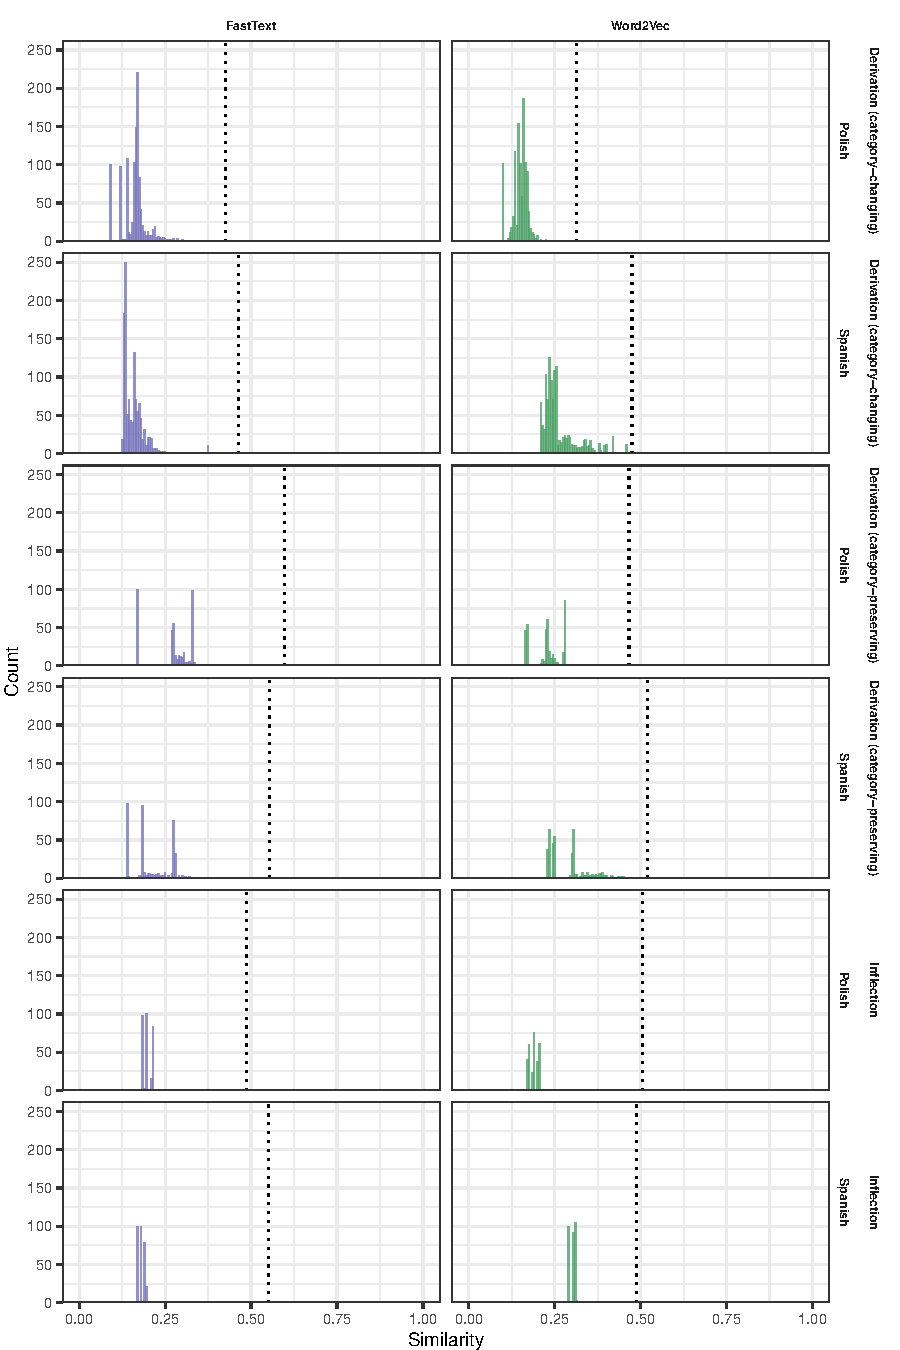
\includegraphics{fig-baseline-faceted.pdf}
\caption{Distribution of the random baseline results. The dotted line represents the mean similarity value on the clean data.}
\label{fig:baseline}
\end{figure}

% \subsection{Statistical analysis}

\section{Results}

\subsection{Clean data}

% CLEAN DATA FIGURE
\begin{figure}[h!]
\centering
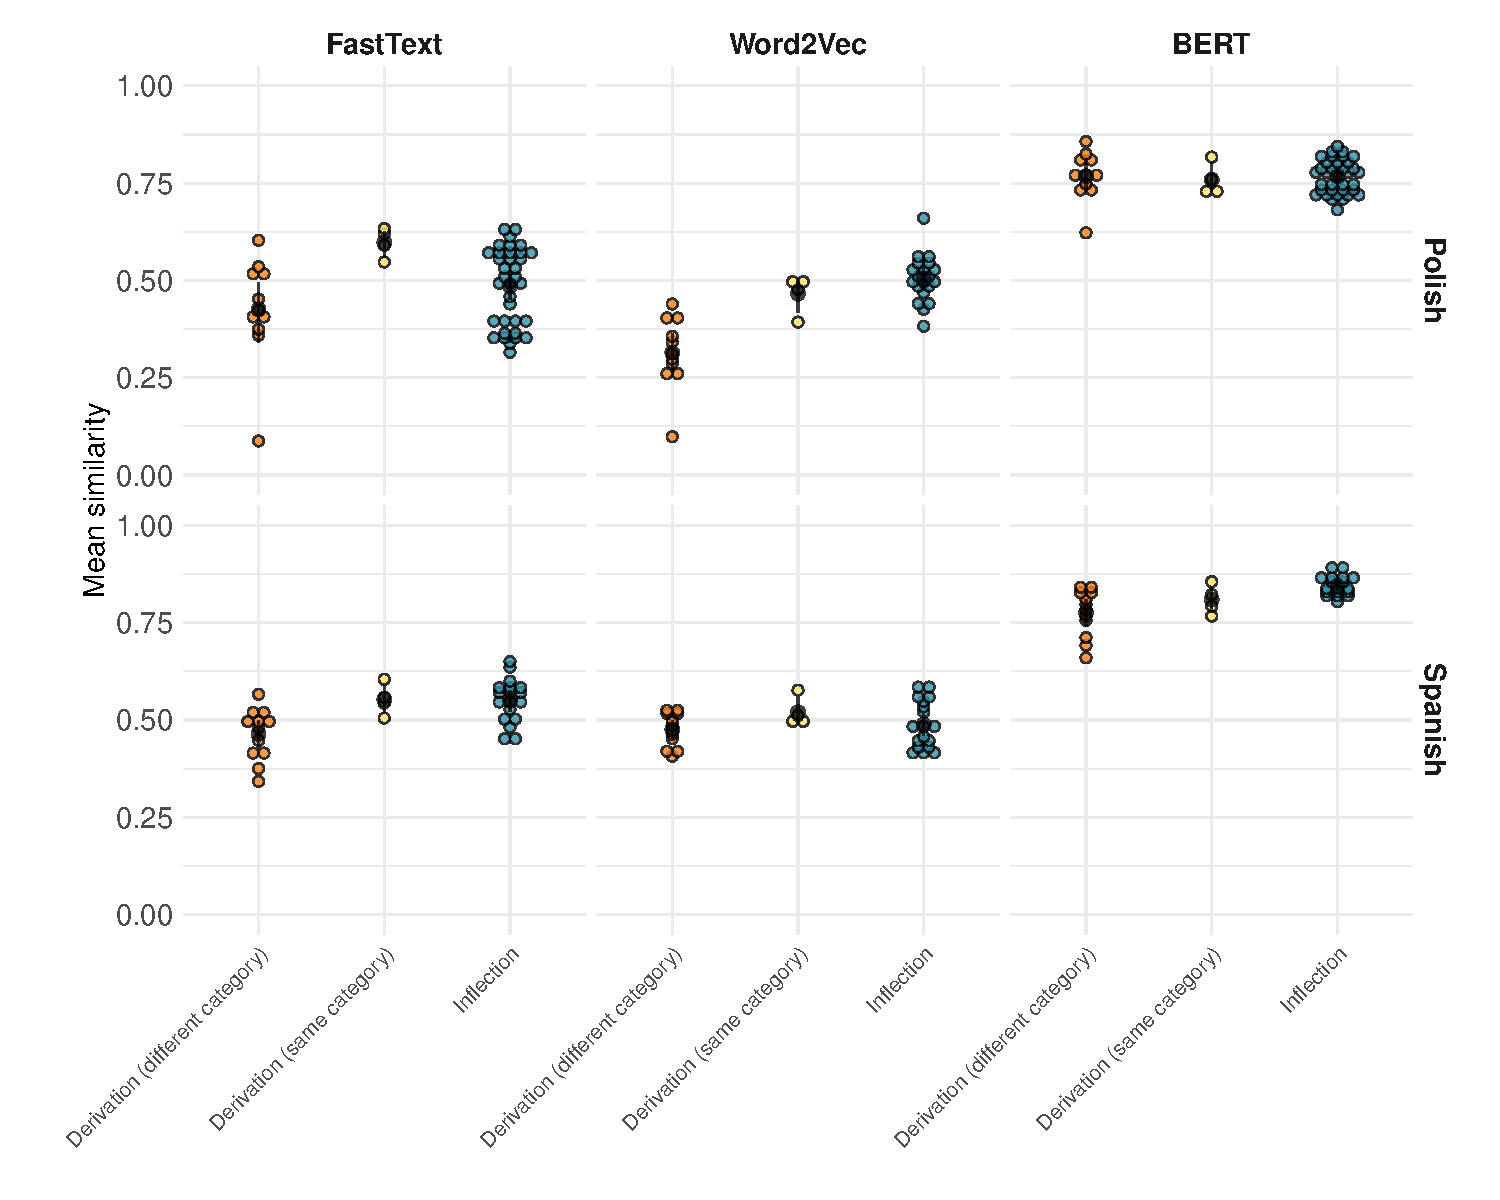
\includegraphics[width=14cm]{fig-clean.pdf}
\caption{Mean similarity between pivot and form in inflection and derivation by model and language. Each dot represents a category. The black dot represents the mean similarity of all the categories and the standard deviation around it.}
\label{fig:clean-data}
\end{figure}

% CLEAN DATA TABLE
\begin{table}[h!]
\centering
\label{tbl:mean-similarity}
\begin{minipage}[t]{0.48\textwidth}
\footnotesize
\centering
\subcaption*{Inflection}
\begin{tabular}{llc}
\toprule
\textbf{Model} & \textbf{Language} & \textbf{Mean similarity} \\
\midrule
\textbf{FastText}  & Spanish & 0.55 \\
                   & Polish  & 0.48 \\
\textbf{Word2Vec}  & Spanish & 0.53 \\
                   & Polish  & 0.51 \\
\bottomrule
\end{tabular}
\end{minipage}
\hfill
\begin{minipage}[t]{0.48\textwidth}
\footnotesize
\centering
\subcaption*{Derivation}
\begin{tabular}{llc}
\toprule
\textbf{Model} & \textbf{Language} & \textbf{Mean similarity} \\
\midrule
\textbf{FastText}  & Spanish & 0.51 \\
                   & Polish  & 0.54 \\
\textbf{Word2Vec}  & Spanish & 0.50 \\
                   & Polish  & 0.40 \\
\bottomrule
\end{tabular}
\end{minipage}
\caption{Mean similarity between pivot and form in inflection and derivation by model and language.}
\end{table}


% \subsection{Subset data}

% \section{Discussion}

% \section{Conclusion}

% Print bibliography
\newpage
\addcontentsline{toc}{section}{References}
\sloppy
\printbibliography
\end{document}
